\documentclass[11pt,compress,t,notes=noshow, xcolor=table]{beamer}
\usepackage[]{graphicx}\usepackage[]{color}
% maxwidth is the original width if it is less than linewidth
% otherwise use linewidth (to make sure the graphics do not exceed the margin)
\makeatletter
\def\maxwidth{ %
  \ifdim\Gin@nat@width>\linewidth
    \linewidth
  \else
    \Gin@nat@width
  \fi
}
\makeatother

\newcommand{\citebutton}[2]{%
\beamergotobutton{\href{#2}{#1}}%
}

\newcommand{\blu}[1]{\textcolor{blue}{#1}}
\newcommand{\org}[1]{\textcolor{orange}{#1}}
\newcommand{\ques}{\textbf{\textcolor{red}{Question:  }}}
\newcommand{\questionssofar}{\begin{frame}\frametitle{Any questions?}\end{frame}}

\newcommand\warning{%
 \makebox[1.4em][c]{%
 \makebox[0pt][c]{\raisebox{.1em}{\scriptsize!}}%
 \makebox[0pt][c]{\color{red}\normalsize$\bigtriangleup$}}}%

\definecolor{fgcolor}{rgb}{0.345, 0.345, 0.345}
\newcommand{\hlnum}[1]{\textcolor[rgb]{0.686,0.059,0.569}{#1}}%
\newcommand{\hlstr}[1]{\textcolor[rgb]{0.192,0.494,0.8}{#1}}%
\newcommand{\hlcom}[1]{\textcolor[rgb]{0.678,0.584,0.686}{\textit{#1}}}%
\newcommand{\hlopt}[1]{\textcolor[rgb]{0,0,0}{#1}}%
\newcommand{\hlstd}[1]{\textcolor[rgb]{0.345,0.345,0.345}{#1}}%
\newcommand{\hlkwa}[1]{\textcolor[rgb]{0.161,0.373,0.58}{\textbf{#1}}}%
\newcommand{\hlkwb}[1]{\textcolor[rgb]{0.69,0.353,0.396}{#1}}%
\newcommand{\hlkwc}[1]{\textcolor[rgb]{0.333,0.667,0.333}{#1}}%
\newcommand{\hlkwd}[1]{\textcolor[rgb]{0.737,0.353,0.396}{\textbf{#1}}}%
\let\hlipl\hlkwb

\usepackage{framed}
\makeatletter
\newenvironment{kframe}{%
 \def\at@end@of@kframe{}%
 \ifinner\ifhmode%
  \def\at@end@of@kframe{\end{minipage}}%
  \begin{minipage}{\columnwidth}%
 \fi\fi%
 \def\FrameCommand##1{\hskip\@totalleftmargin \hskip-\fboxsep
 \colorbox{shadecolor}{##1}\hskip-\fboxsep
     % There is no \\@totalrightmargin, so:
     \hskip-\linewidth \hskip-\@totalleftmargin \hskip\columnwidth}%
 \MakeFramed {\advance\hsize-\width
   \@totalleftmargin\z@ \linewidth\hsize
   \@setminipage}}%
 {\par\unskip\endMakeFramed%
 \at@end@of@kframe}
\makeatother

\definecolor{shadecolor}{rgb}{.97, .97, .97}
\definecolor{messagecolor}{rgb}{0, 0, 0}
\definecolor{warningcolor}{rgb}{1, 0, 1}
\definecolor{errorcolor}{rgb}{1, 0, 0}
\newenvironment{knitrout}{}{} % an empty environment to be redefined in TeX

\usepackage{alltt}
\newcommand{\SweaveOpts}[1]{}  % do not interfere with LaTeX
\newcommand{\SweaveInput}[1]{} % because they are not real TeX commands
\newcommand{\Sexpr}[1]{}       % will only be parsed by R
\newcommand{\xmark}{\ding{55}}%


\usepackage[english]{babel}
\usepackage[utf8]{inputenc}

\usepackage{dsfont}
\usepackage{verbatim}
\usepackage{amsmath}
\usepackage{amsfonts}
\usepackage{amssymb}
\usepackage{bm}
\usepackage{csquotes}
\usepackage{multirow}
\usepackage{longtable}
\usepackage{booktabs}
\usepackage{enumerate}
\usepackage[absolute,overlay]{textpos}
\usepackage{psfrag}
\usepackage{algorithm}
\usepackage{algpseudocode}
\usepackage{eqnarray}
\usepackage{arydshln}
\usepackage{tabularx}
\usepackage{placeins}
\usepackage{tikz}
\usepackage{setspace}
\usepackage{colortbl}
\usepackage{mathtools}
\usepackage{wrapfig}
\usepackage{bm}
\usepackage{amsmath}
\usepackage{pifont}

\usetikzlibrary{shapes.multipart,shapes,arrows,automata,positioning,calc,chains,trees, shadows}
\tikzset{
  %Define standard arrow tip
  >=stealth',
  %Define style for boxes
  punkt/.style={
    rectangle,
    rounded corners,
    draw=black, very thick,
    text width=6.5em,
    minimum height=2em,
    text centered},
  % Define arrow style
  pil/.style={
    ->,
    thick,
    shorten <=2pt,
    shorten >=2pt,}
}

\tikzstyle{vec}=[draw, rectangle, fill = white, minimum width=5mm, minimum height=1cm, inner sep = 2pt]

\usepackage{subfig}

% Defines macros and environments
\usepackage{../../style/lmu-lecture}


\let\code=\texttt
\let\proglang=\textsf

\setkeys{Gin}{width=0.9\textwidth}

\setbeamertemplate{frametitle}{\expandafter\uppercase\expandafter\insertframetitle}

\usepackage{bbm}
% basic latex stuff
\newcommand{\pkg}[1]{{\fontseries{b}\selectfont #1}} %fontstyle for R packages
\newcommand{\lz}{\vspace{0.5cm}} %vertical space
\newcommand{\dlz}{\vspace{1cm}} %double vertical space
\newcommand{\oneliner}[1] % Oneliner for important statements
{\begin{block}{}\begin{center}\begin{Large}#1\end{Large}\end{center}\end{block}}


%new environments
\newenvironment{vbframe}  %frame with breaks and verbatim
{
 \begin{frame}[containsverbatim,allowframebreaks]
}
{
\end{frame}
}

\newenvironment{vframe}  %frame with verbatim without breaks (to avoid numbering one slided frames)
{
 \begin{frame}[containsverbatim]
}
{
\end{frame}
}

\newenvironment{blocki}[1]   % itemize block
{
 \begin{block}{#1}\begin{itemize}
}
{
\end{itemize}\end{block}
}

\newenvironment{fragileframe}[2]{  %fragile frame with framebreaks
\begin{frame}[allowframebreaks, fragile, environment = fragileframe]
\frametitle{#1}
#2}
{\end{frame}}


\newcommand{\myframe}[2]{  %short for frame with framebreaks
\begin{frame}[allowframebreaks]
\frametitle{#1}
#2
\end{frame}}

\newcommand{\remark}[1]{
  \textbf{Remark:} #1
}


\newenvironment{deleteframe}
{
\begingroup
\usebackgroundtemplate{
\includegraphics[width=\paperwidth,height=\paperheight]{../style/color/red.png}}
 \begin{frame}
}
{
\end{frame}
\endgroup
}
\newenvironment{simplifyframe}
{
\begingroup
\usebackgroundtemplate{
\includegraphics[width=\paperwidth,height=\paperheight]{../style/color/yellow.png}}
 \begin{frame}
}
{
\end{frame}
\endgroup
}\newenvironment{draftframe}
{
\begingroup
\usebackgroundtemplate{
\includegraphics[width=\paperwidth,height=\paperheight]{../style/color/green.jpg}}
 \begin{frame}
}
{
\end{frame}
\endgroup
}
% https://tex.stackexchange.com/a/261480: textcolor that works in mathmode
\makeatletter
\renewcommand*{\@textcolor}[3]{%
  \protect\leavevmode
  \begingroup
    \color#1{#2}#3%
  \endgroup
}
\makeatother





\input{../../latex-math/basic-math.tex}
\input{../../latex-math/basic-ml.tex}

%\newcommand{\titlefigure}{figure/gpt_sq.png}
\newcommand{\learninggoals}{
\item Understand Chinchilla
\item Understand the various scaling laws
}
\definecolor{texblue}{rgb}{0, 0, 1}
\def\myblue#1{\textcolor{texblue}{#1}}

\title{Training Large Language Models}
% \author{}
\institute{\href{https://slds-lmu.github.io/lecture_dl4nlp/}{slds-lmu.github.io/lecture\_dl4nlp}}
\date{}

\begin{document}
\lecturechapter{Scaling Laws and Chinchilla}
\lecture{Deep Learning for NLP}


%Notes:
% Slides: https://jasonwei20.github.io/files/FLAN%20talk%20external.pdf
% Check out emergence talk: https://www.youtube.com/watch?v=0SuyDLjNR9g

% LLM Survey: https://arxiv.org/pdf/2303.18223.pdf

% ------------------------------------------------------------------------------

\begin{vbframe}{Number of Parameters: Notation}

\vfill

\begin{itemize}
    \item Up to now in this chapter: number of parameters = $P$
    \item From now on: number of parameters = $N$
\end{itemize}

\vfill
    
\end{vbframe}

% ------------------------------------------------------------------------------

\begin{vbframe}{Scaling Laws Proposed by Kaplan et al. (2020)}
\href{https://arxiv.org/abs/2001.08361}{\beamergotobutton{Kaplan et al. (2020)}} 

\vfill

\begin{itemize}

	\item Performance depends strongly on scale, weakly on model shape
	\begin{itemize}
	\item Scale means: parameters $N$, data $D$, and compute $C$
	\item Shape means: depth and width
	\end{itemize}

	\item Smooth power laws
	\begin{itemize}
	\item Performance has power-law relation with each factor $N$, $D$, $C$
	\item When not bottlenecked by the other two 
	\item Trend spanning more than six orders of magnitude
	\end{itemize}

	\item Universality of overfitting 
	\begin{itemize}
	\item Performance enters regime of diminishing returns if $N$ or $D$ held fixed while the other increases
	\end{itemize}

\end{itemize}

\vfill

\end{vbframe}

% ------------------------------------------------------------------------------

\begin{vbframe}{Scaling Laws Proposed by Kaplan et al. (2020)}

\vfill

\begin{itemize}

	\item Universality of training
	\begin{itemize}
	\item Training curves follow predictable power-laws
	\item Their parameters are roughly independent of model size
	\item It is possible to predict by extrapolating the early part of the training curve
	\end{itemize}

	\item Transfer improves with test performance
	\begin{itemize}
	\item When evaluating on text with different distribution from training text, results are strongly correlated to those on the validation set
	\item Transfer to different distribution incurs a constant penalty but improves in line with performance on training set
	\end{itemize}

	\item Sample efficiency
	\begin{itemize}
	\item Large models are more sample-efficient than small models
	\item They reach same performance with fewer optimization steps
	\end{itemize}

\end{itemize}

\vfill

\end{vbframe}

% ------------------------------------------------------------------------------

\begin{vbframe}{Power Law (GPT3 Paper)}

\begin{figure}
    \centering
    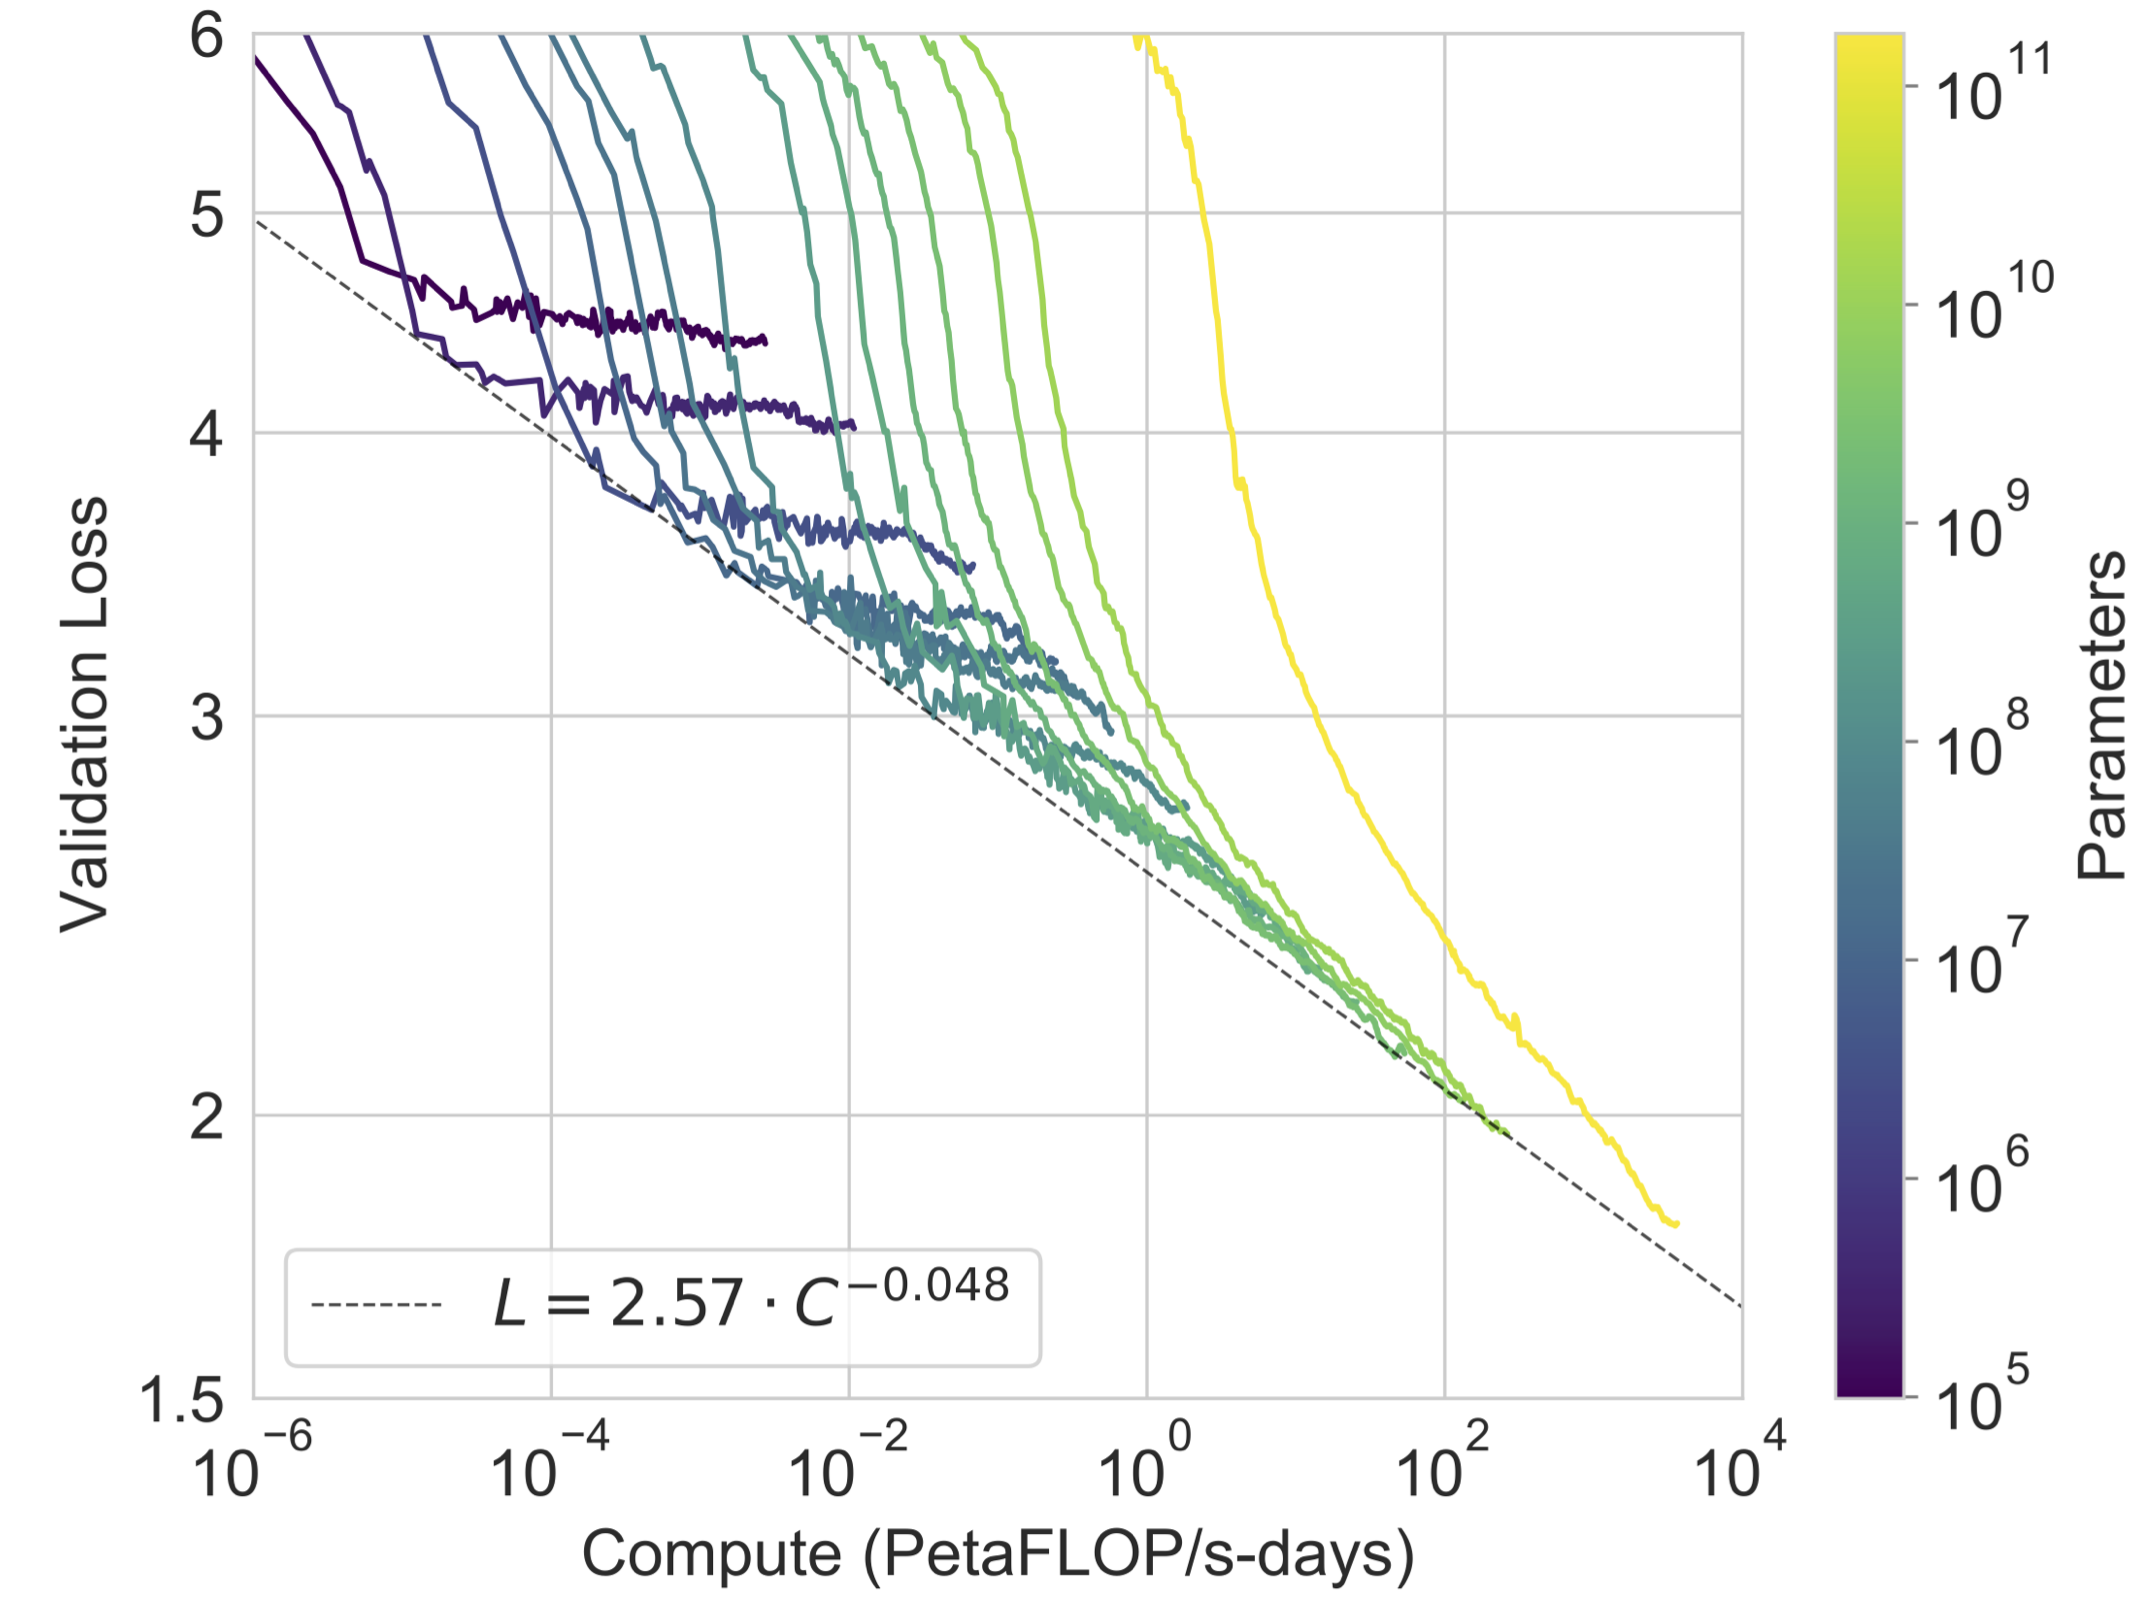
\includegraphics[width=10cm]{figure/losscompute.png}
\end{figure}
    
\end{vbframe}

% ------------------------------------------------------------------------------

\begin{vbframe}{Scaling Laws}

\vfill

\begin{itemize}

	\item Convergence is inefficient
	\begin{itemize}
	\item When $C$ is fixed but $N$ and $D$ are not, optimal performance is achived by training very large models and stopping significantly short of convergence  
	\end{itemize}

	\item Optimal batch size
	\begin{itemize}
    	\item Claim: “Optimal batch size: The ideal batch size for training these
                models is roughly a power of the loss only, and continues to
                be determinable by measuring the gradient noise scale
                [MKAT18]; it is roughly 1-2 million tokens at convergence for
                the largest models we can train.”
    	\item gradient noise scale = a measure of the signal-to-noise ratio
            of gradient across training examples
	\end{itemize}

\end{itemize}

\vskip3mm

\textbf{Claim: Larger language models will perform better and be more sample efficient than current models.} 

\vfill

\end{vbframe}

% ------------------------------------------------------------------------------

\begin{vbframe}{Optimal Batch Size}

\begin{figure}
    \centering
    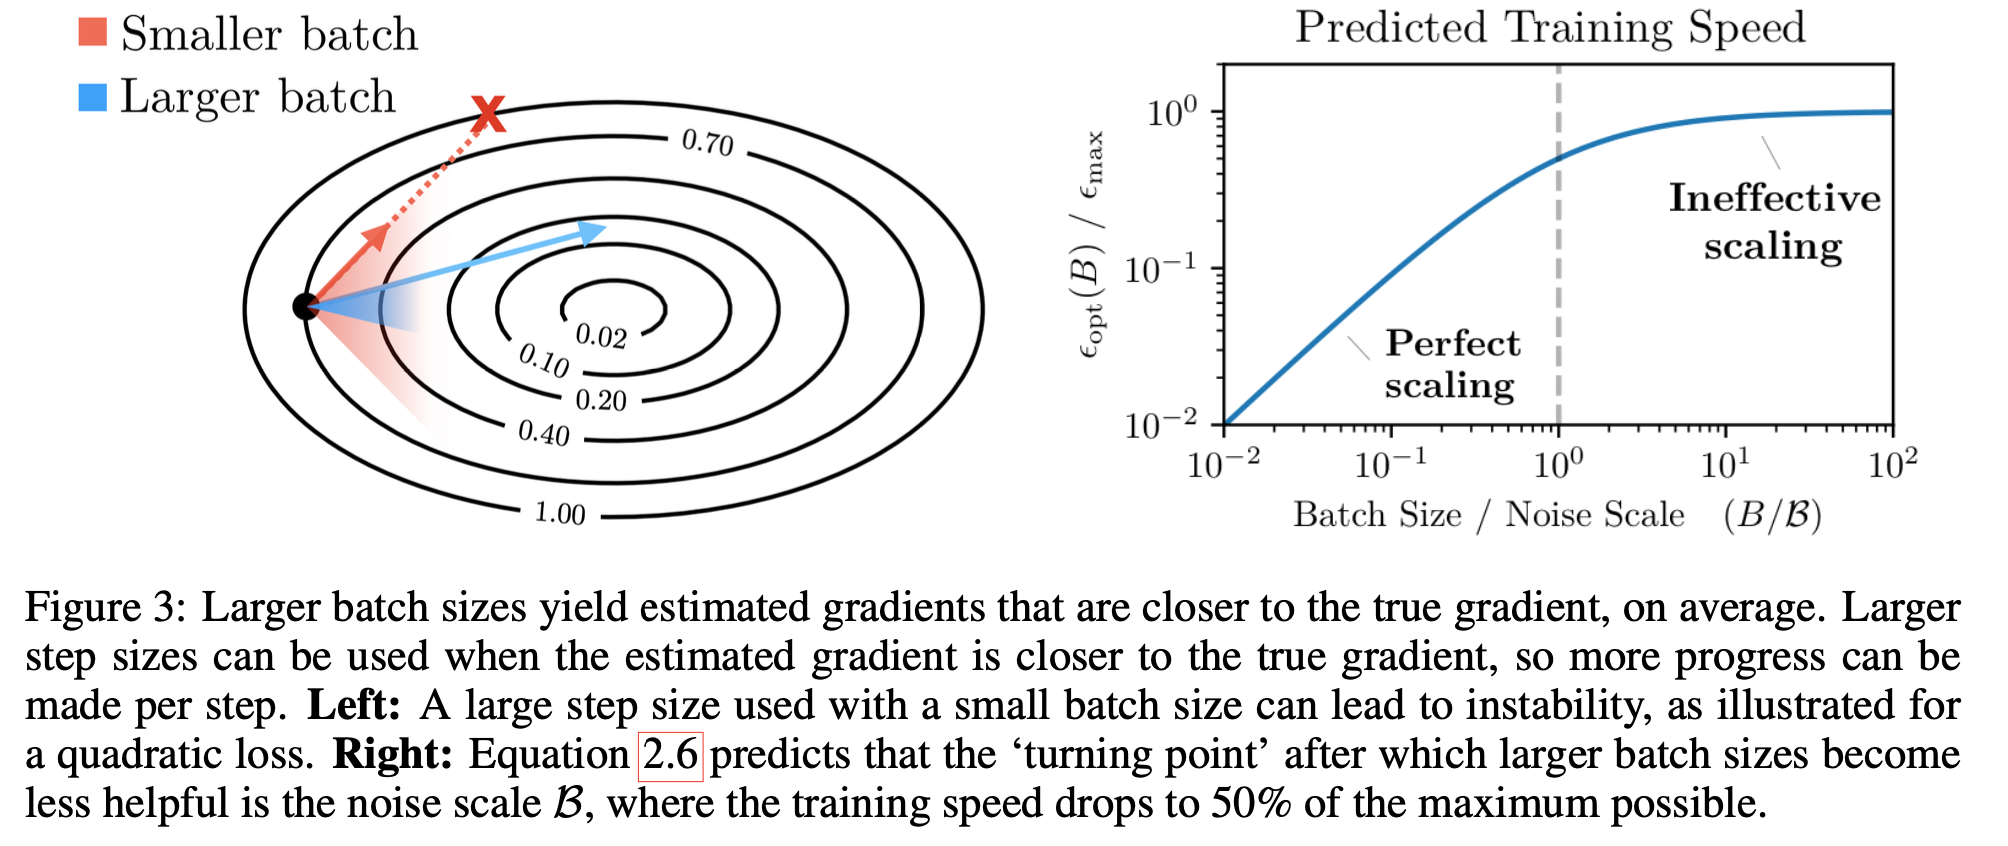
\includegraphics[height = 6cm]{figure/optimalbatchsize.png}
\end{figure}


\end{vbframe}

\begin{vbframe}{Optimal Batch Size}

\begin{figure}
    \centering
    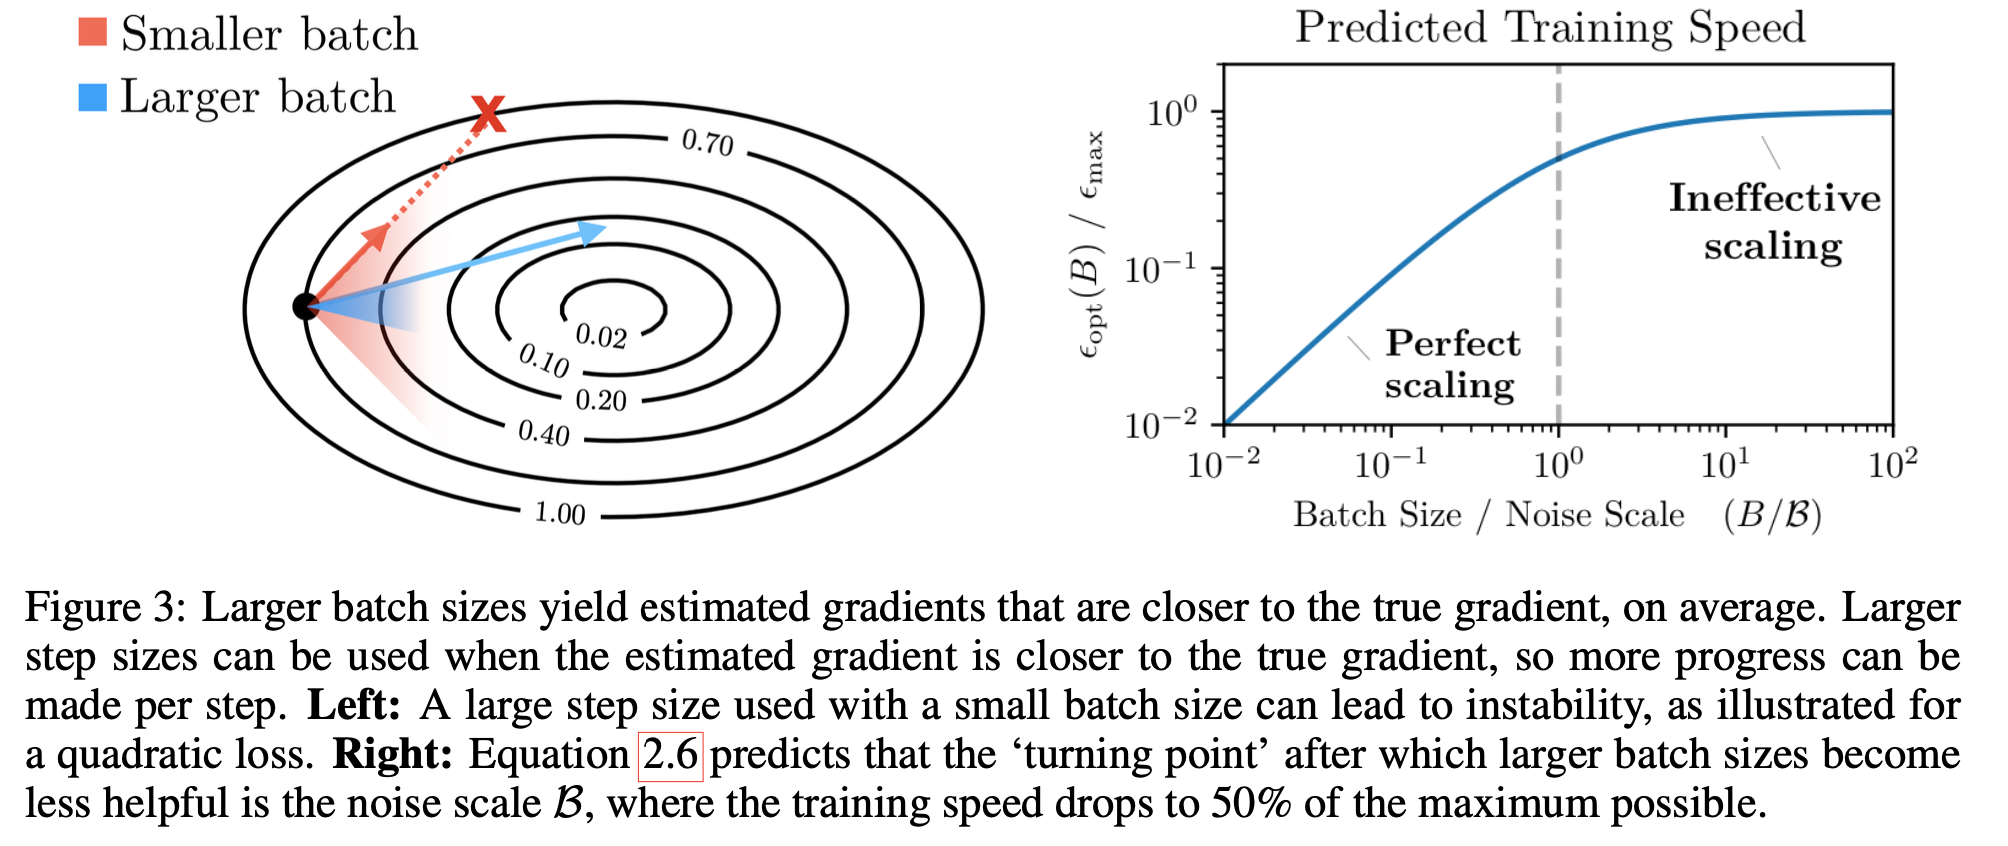
\includegraphics[height = 3cm]{figure/optimalbatchsize.png}
\end{figure}

\begin{itemize}
    \item Estimate gradient as accurately as possible $\rightarrow$ large batch
    \item Increase training speed as much as possible $\rightarrow$ large step size
    \item Based on the estimated gradient, choose a step size such that the cost of the landing position does not deviate too much from the cost of the ideal landing position $\rightarrow$ small step size
    \item Exploit stochasticity (epoch batches would not be a good thing even if we could compute them efficiently) $\rightarrow$ small step size

\end{itemize}

\end{vbframe}

% ------------------------------------------------------------------------------

\begin{vbframe}{Scaling Law for next word prediction}

\vfill

\begin{itemize}
    \item $L(N,D) = 1.61 + \frac{406.4}{N^{0.34}} + \frac{410.7}{D^{0.28}}$
    \item $L(N,D)$ is cross entropy on new text
\end{itemize}

\vfill

\end{vbframe}

% ------------------------------------------------------------------------------

\begin{vbframe}{Compute-Optimal LLM\MakeLowercase{s}}

Given a fixed FLOPs budget, how should we trade-off model size and text size to optimize performance? \citebutton{Hoffmann et al., 2022}{https://arxiv.org/abs/2203.15556}

\vfill

\begin{itemize}

	\item Find $N$ and $D$ so that $FLOPs(N,D) = C$ and $L(N,D)$ is minimal

	\item Empirically estimated $N$ and $D$ based on 400 models. 
	\begin{itemize}
	\item Ranging from 70\,M to 16\,B parameters
	\item Trained on 5\,B to 400\,B tokens
	\end{itemize}

	\item Different results from those of \citebutton{Kaplan et al., 2020}{https://arxiv.org/abs/2001.08361} 
	\item Results verified using Chinchilla
	\begin{itemize}
	\item Chinchilla has 70\,B parameters and is trained on 1.4\,T tokens
	\item 4x less parameters and 4x more tokens than Gopher
	\item Chinchilla outruns Gopher and has reduced memory footprint and inference cost 
	\end{itemize}

\end{itemize}

\vfill

\end{vbframe}

% ------------------------------------------------------------------------------

\begin{vbframe}{Compute-Optimal LLM\MakeLowercase{s}: Are GPT3 etc too large?}

\vfill

\begin{figure}
	\centering
	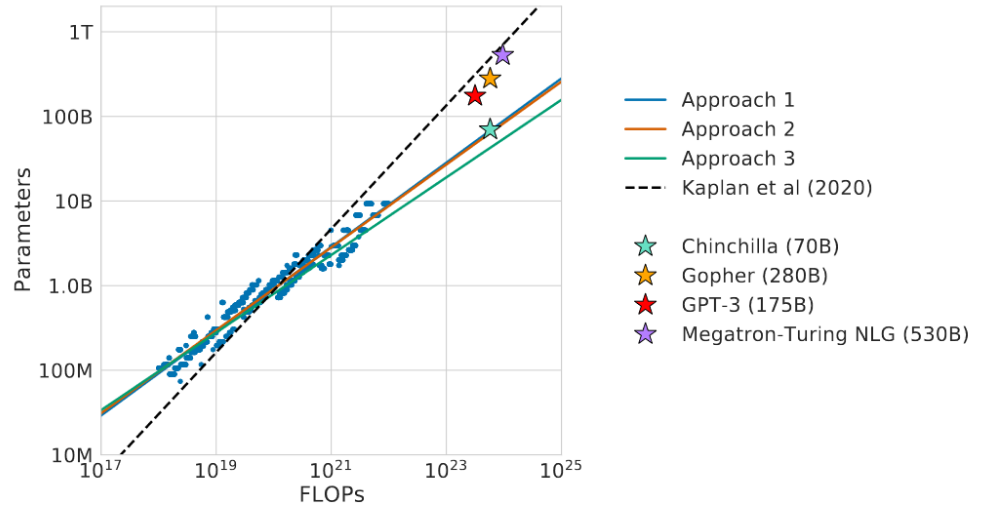
\includegraphics[width = 11cm]{./figure/chinchilla.png} \\ 
	\citebutton{Source: Hoffmann et al., 2022}{https://arxiv.org/abs/2203.15556}
\end{figure}

\vfill

\end{vbframe}

% ------------------------------------------------------------------------------

\begin{vbframe}{Compute-Optimal LLM\MakeLowercase{s} (2)}

Given a fixed FLOPs budget, how should one trade off model size and
the number of training tokens? We find that all three methods predict
that current large models should be substantially smaller and therefore
trained much longer than is currently done. Based on our estimated
compute-optimal frontier, we predict that for the compute budget used
to train Gopher, an optimal model should be 4 times smaller, while
being training on 4 times more tokens. We verify this by training a more
compute-optimal 70B model, called Chinchilla, on 1.4 trillion tokens.
Not only does Chinchilla outperform its much larger counterpart,
Gopher, but its reduced model size reduces inference cost considerably
and greatly facilitates downstream uses on smaller hardware. The
energy cost of a large language model is amortized through its usage
for inference and fine-tuning. The benefits of a more optimally trained
smaller model, therefore, extend beyond the immediate benefits of its
improved performance.

\end{vbframe}

% ------------------------------------------------------------------------------

\begin{vbframe}{Chinchilla and the other LLM\MakeLowercase{s}}

\vfill

\begin{figure}
	\centering
	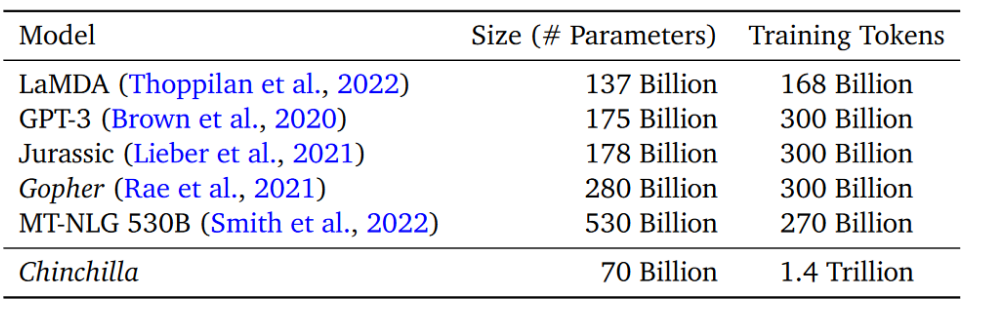
\includegraphics[width = 11cm]{./figure/llm_params.png} \\ 
	\citebutton{Source: Hoffmann et al., 2022}{https://arxiv.org/abs/2203.15556}
\end{figure}

\begin{figure}
	\centering
	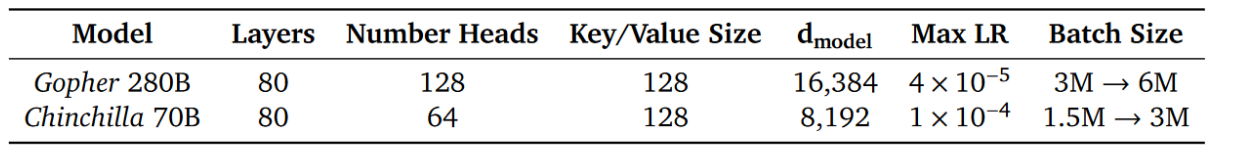
\includegraphics[width = 11cm]{./figure/chinchilla_gopher.png} \\ 
	\citebutton{Source: Hoffmann et al., 2022}{https://arxiv.org/abs/2203.15556}
\end{figure}

\vfill

\end{vbframe}

% ------------------------------------------------------------------------------

\begin{vbframe}{Chinchilla outperforms other LLM\MakeLowercase{s}: MMLU}

\vfill

\begin{figure}
	\centering
	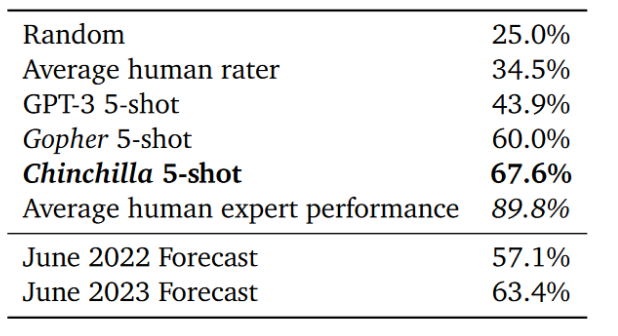
\includegraphics[width = 8cm]{./figure/chinchilla_mmlu.png} \\ 
	\citebutton{Source: Hoffmann et al., 2022}{https://arxiv.org/abs/2203.15556}
\end{figure}

\vfill

\end{vbframe}

% ------------------------------------------------------------------------------

\begin{vbframe}{Chinchilla outperforms other LLM\MakeLowercase{s}: QA}

\vfill

\begin{figure}
	\centering
	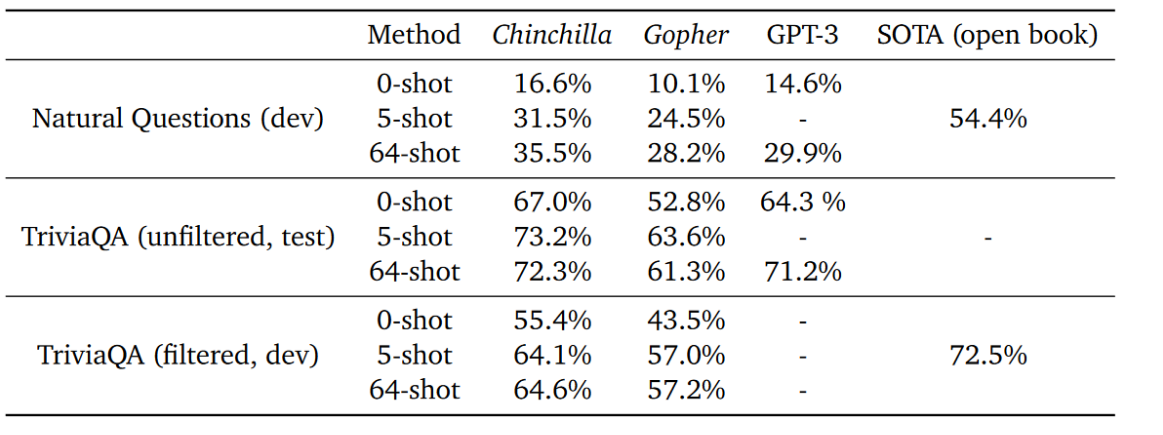
\includegraphics[width = 12cm]{./figure/chinchilla_qa.png} \\ 
	\citebutton{Source: Hoffmann et al., 2022}{https://arxiv.org/abs/2203.15556}
\end{figure}

\vfill

\end{vbframe}

% ------------------------------------------------------------------------------

\begin{vbframe}{Scaling laws: Discussion}

\vfill

\begin{figure}
	\centering
	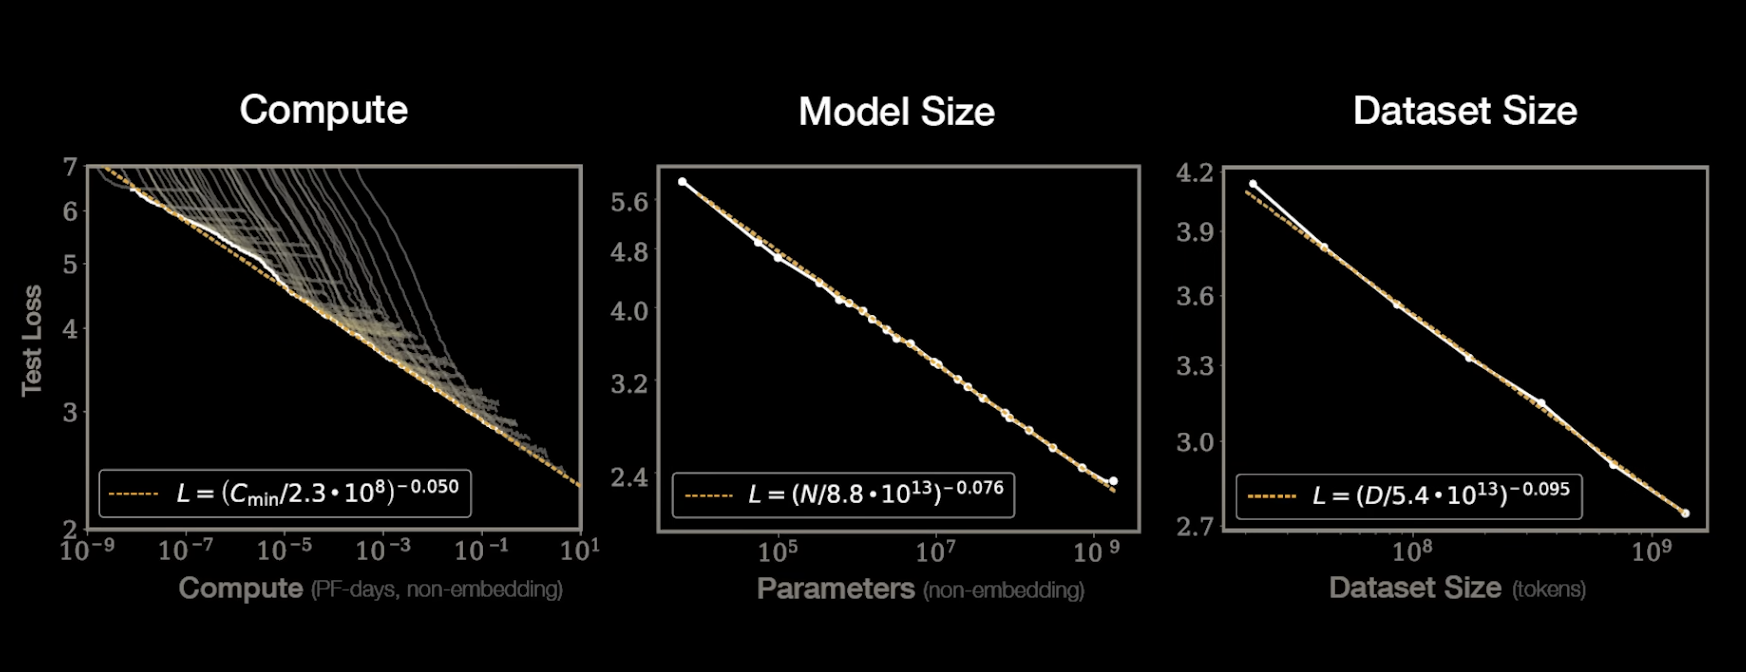
\includegraphics[width = 11cm]{./figure/3thingserrorratescaleswith.png} \\ 
\end{figure}

\ques Any doubts?

\vfill

% do we have enough text?
% do we have enough compute?
% can we afford that much compute?
% Sutskever: results from scaling up pretraining
% have plateaued
% Sutskever: scaling the right thing matters more now than ever
% the verge 20241025: gemini
% not showing performacne that the deepmind team had hoped
% for
% general trend in the audience?
% https://www.theverge.com/2024/10/25/24279600/google-next-gemini-ai-model-openai-december
% ai companies cannot really say that scaling is notw orkgin
% because valuation depends on that

\end{vbframe}

% ------------------------------------------------------------------------------


\begin{vbframe}{Doubts about scaling (1)}

\vfill

\begin{itemize}
\item \citebutton{Reuters}{https://www.reuters.com/technology/artificial-intelligence/openai-rivals-seek-new-path-smarter-ai-current-methods-hit-limitations-2024-11-11/}
\begin{itemize}
\item Ilya Sutskever, co-founder of AI labs Safe Superintelligence
	(SSI) and OpenAI, told Reuters recently that results
	from scaling up pre-training -- the phase of training
	an AI model that uses a vast amount of unlabeled
	data to understand language patterns and structures
	-- have plateaued.
	\item
But now, some of the most prominent AI scientists are
speaking out on the limitations of this “bigger is better”
philosophy.
\item “The 2010s were the age of scaling, now we're back in
	the age of wonder and discovery once again. Everyone
	is looking for the next thing,” Sutskever
	said. “Scaling the right thing matters more now than ever.”
\end{itemize}
\end{itemize}


\vfill

\end{vbframe}


\begin{vbframe}{Doubts about scaling (2)}

\vfill

\begin{itemize}
\item \citebutton{The Verge}{https://www.theverge.com/2024/10/25/24279600/google-next-gemini-ai-model-openai-december}
\begin{itemize}
\item I've heard that the model (December Gemini release) isn't showing the
	performance
        gains the Demis Hassabis-led team had hoped for \ldots
\end{itemize}
\item Andrew Ng's news letter:
``Orion’s improvement over GPT-4 was
far smaller than that from GPT-3 to GPT-4.'',
``OpenAI found that pretraining Orion on
synthetic data made it too much like earlier models \ldots'',
``Anthropic’s schedule for \ldots\ Claude 3.5 Opus \ldots\
has slipped. It
hasn’t shown the expected performance given its size and
cost \ldots'',
\end{itemize}


\vfill

\end{vbframe}

\begin{vbframe}{Epoch AI projections}

\vfill

\begin{figure}
	\centering
	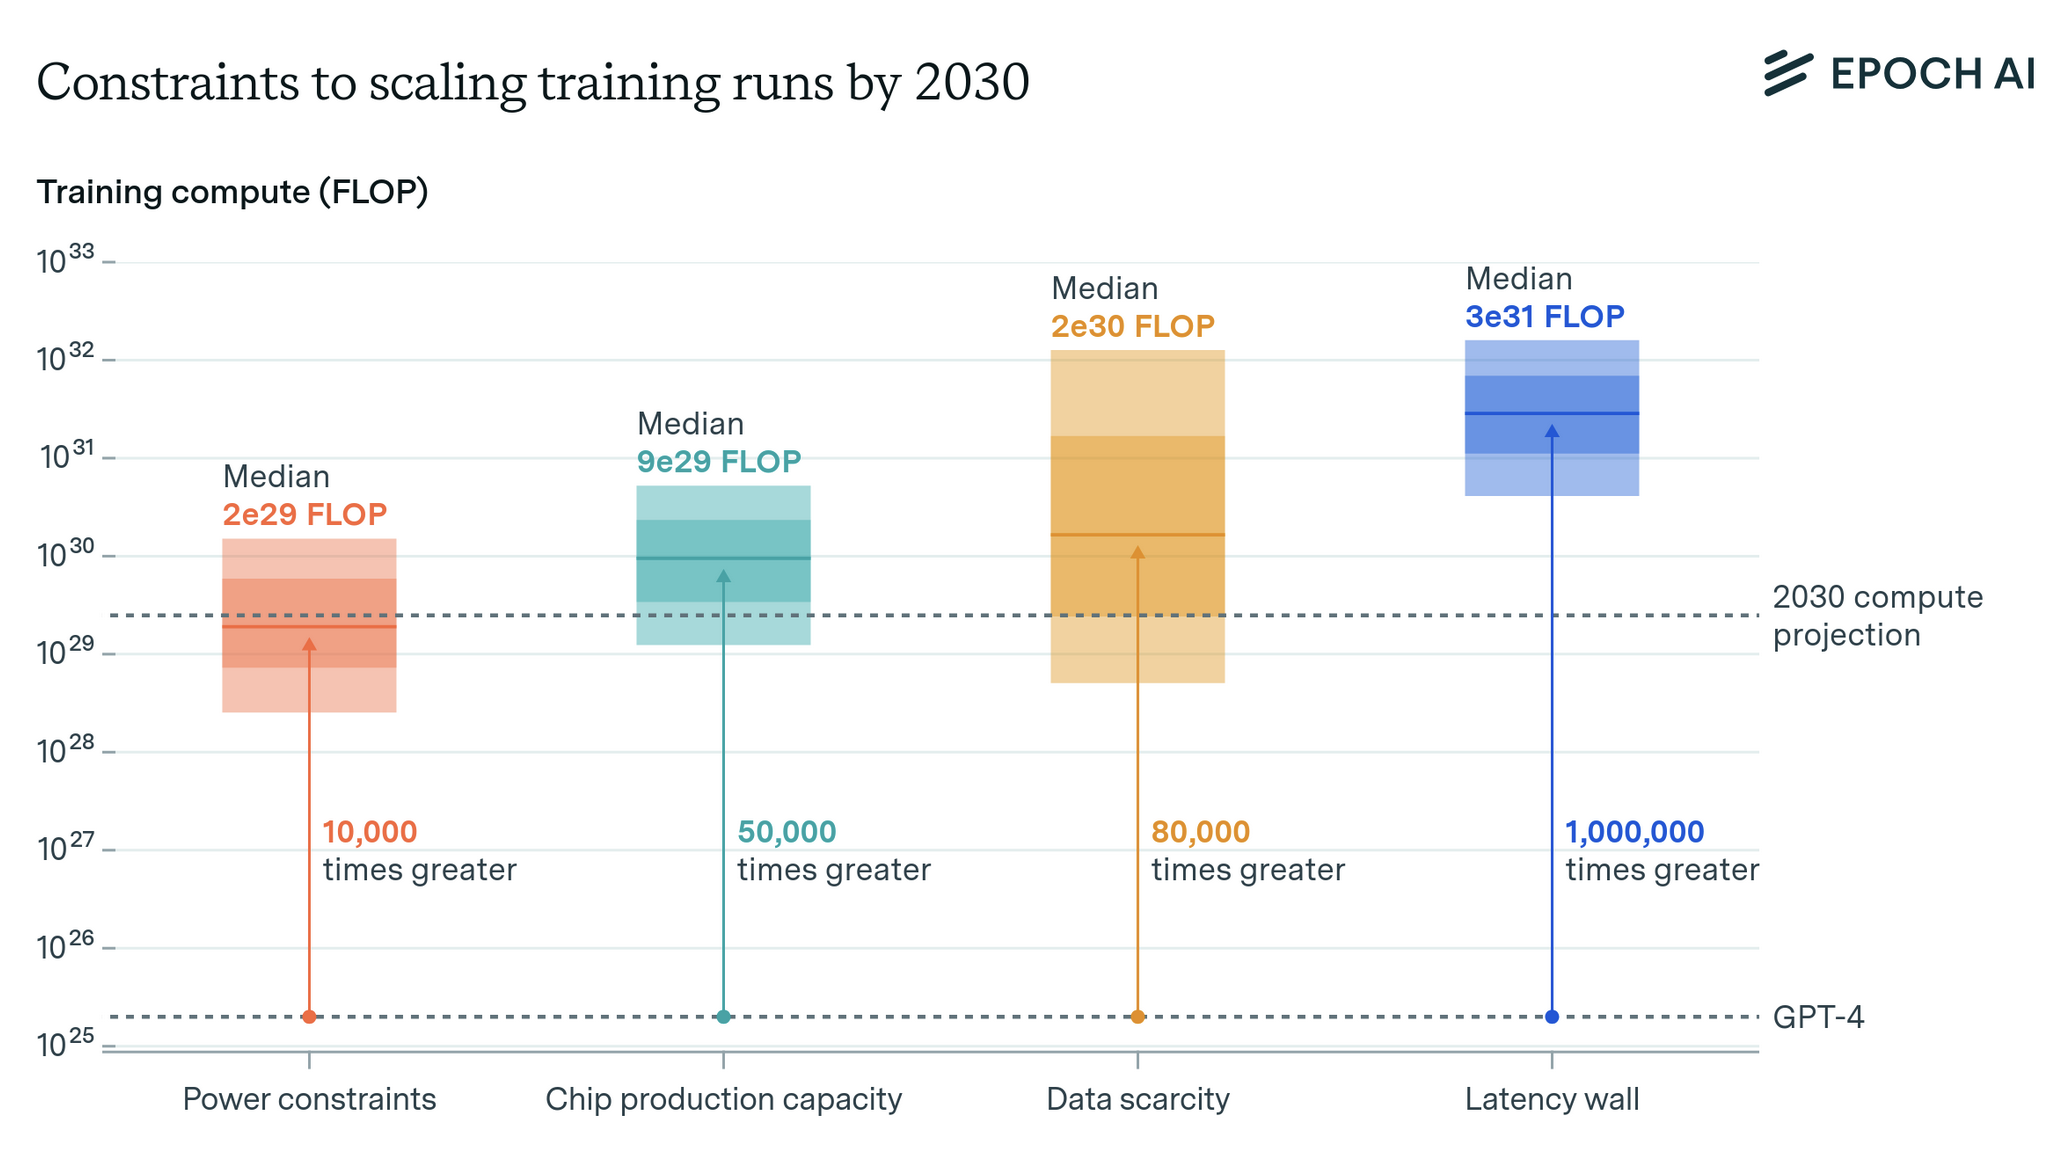
\includegraphics[height = 6cm]{./figure/epochai.png} 
\end{figure}

\citebutton{Epoch AI}{https://epoch.ai/blog/can-ai-scaling-continue-through-2030}


\vfill

\end{vbframe}


\begin{vbframe}{It's not simply brute-force scaling (1)}

\vfill

\begin{itemize}
	\item Data
	\begin{itemize}
	\item If you run out of data, then increase \# epochs
        \item The Stack v2
	already contais all public code! arxiv.org/abs/2305.16264
        \item data quality/model size tradeoff: Training
	a smaller model on  a smaller high-quality dataset may be
	better than trainig a huge model on a huge
	medium-quality dataset.
        \item For higher quality datasets, allocate more
	compute to model size. arxiv.org/abs/2401.02954
        \item See Stanford CS25: StarCoder Use Case
	\end{itemize}

\end{itemize}

\vfill

\end{vbframe}


\begin{vbframe}{It's not simply brute-force scaling (2)}

\vfill

\begin{itemize}
	\item Scaling laws ignore cost per (input/output) token 
	\begin{itemize}
	\item Even if a humongous model gives me the best
	possible performance, cost per token may be
	prohibitively expensive.
        \item Example: Llama models are small-ish because
	that's the size that makes economic sense right now.
        \item huge openai models may not make economic sense
        \item The
        latest models cost as much as \$100 million to train,
	and
        this number could reach \$100 billion within a few
	years,
        according to Anthropic’s Dario Amodei. Rising costs
	could
        lead companies to reallocate their gargantuan
	training
        budgets and researchers to focus on more
	cost-effective,
        application-specific approaches. (Andrew Ng)
         
	\end{itemize}

\end{itemize}

\vfill

\end{vbframe}


\begin{vbframe}{Phi-4}

\vfill

\begin{itemize}
\item release by Microsoft Dec 2024
	\item 14 billion parameters (small!)
	\item pretraining data: 9.8 trillion tokens
        \item pretraining data curated / synthesized
\end{itemize}

\vfill

\end{vbframe}


\begin{vbframe}{Scaling: Train/test tradeoff}

\vfill

\begin{figure}
	\centering
	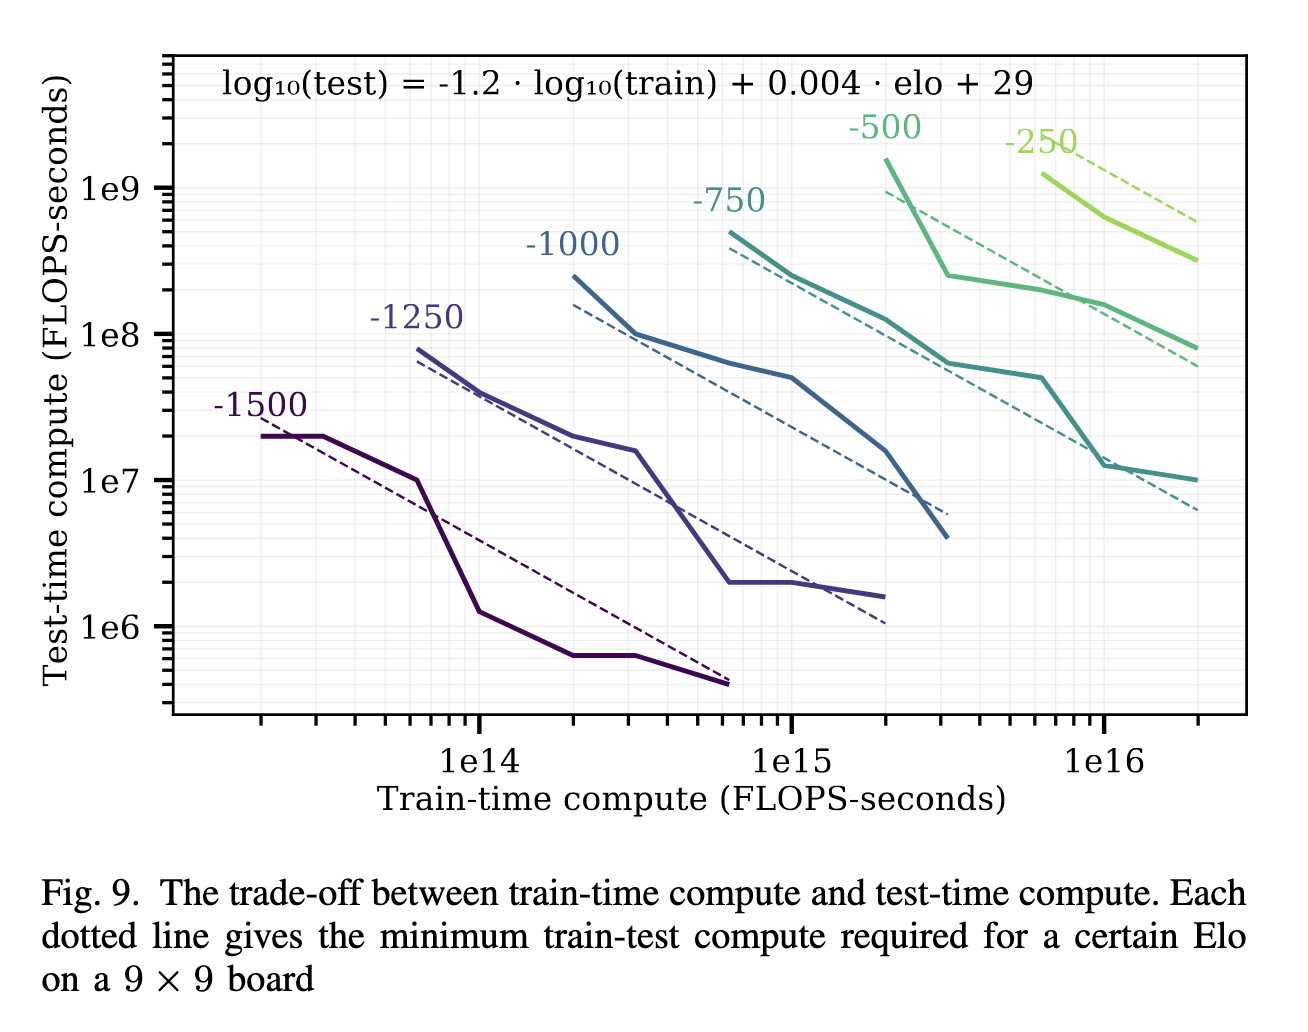
\includegraphics[height = 6cm]{./figure/scalingtraintest.png} \\ 
\end{figure}

\citebutton{Andy L. Jones}{https://arxiv.org/abs/2104.03113}
                 
\vfill



\end{vbframe}


\begin{vbframe}{Shift away from scaling towards test time /
	systems approaches}

\vfill

\begin{itemize}
	\item When investing more test-time compute, small
	models can outperform much larger models
        \citebutton{Snell et al}{https://arxiv.org/pdf/2408.03314v1}
\item Many recent innovations (all implemented in o1?) were not about scaling.
\begin{itemize}
\item Train on synthetic data (e.g., chain of thought)
\item Reflection
\item Test-time adaptation
\end{itemize}

\item Focus more on compound/integrated systems with many
smaller components rather than a single gargantuan
end-to-end monolithic model.
\end{itemize}

\vfill

\end{vbframe}


\begin{vbframe}{If there's one thing you should take away (1)}

\vfill

\begin{figure}
	\centering
	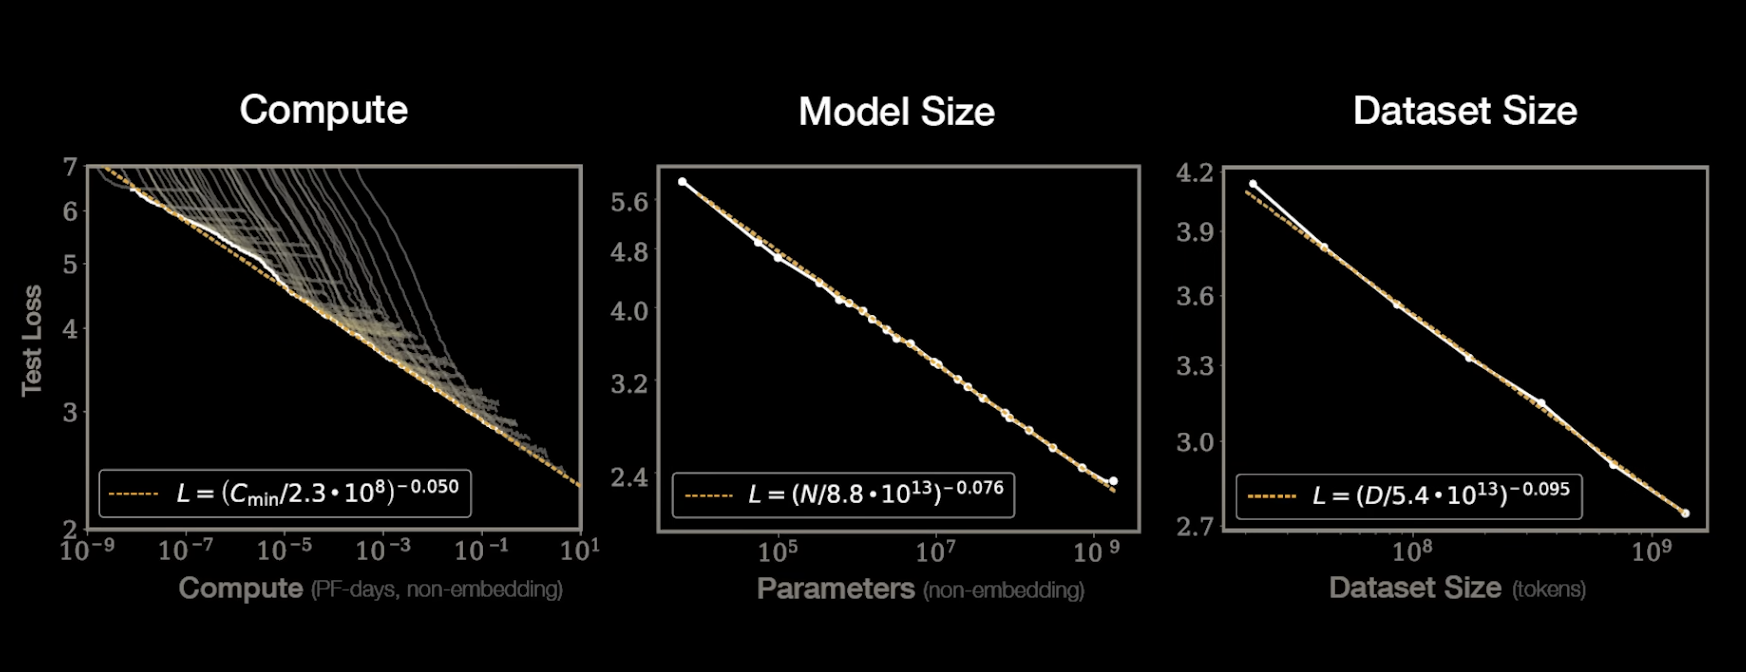
\includegraphics[width = 12cm]{./figure/3thingserrorratescaleswith.png} \\ 
%	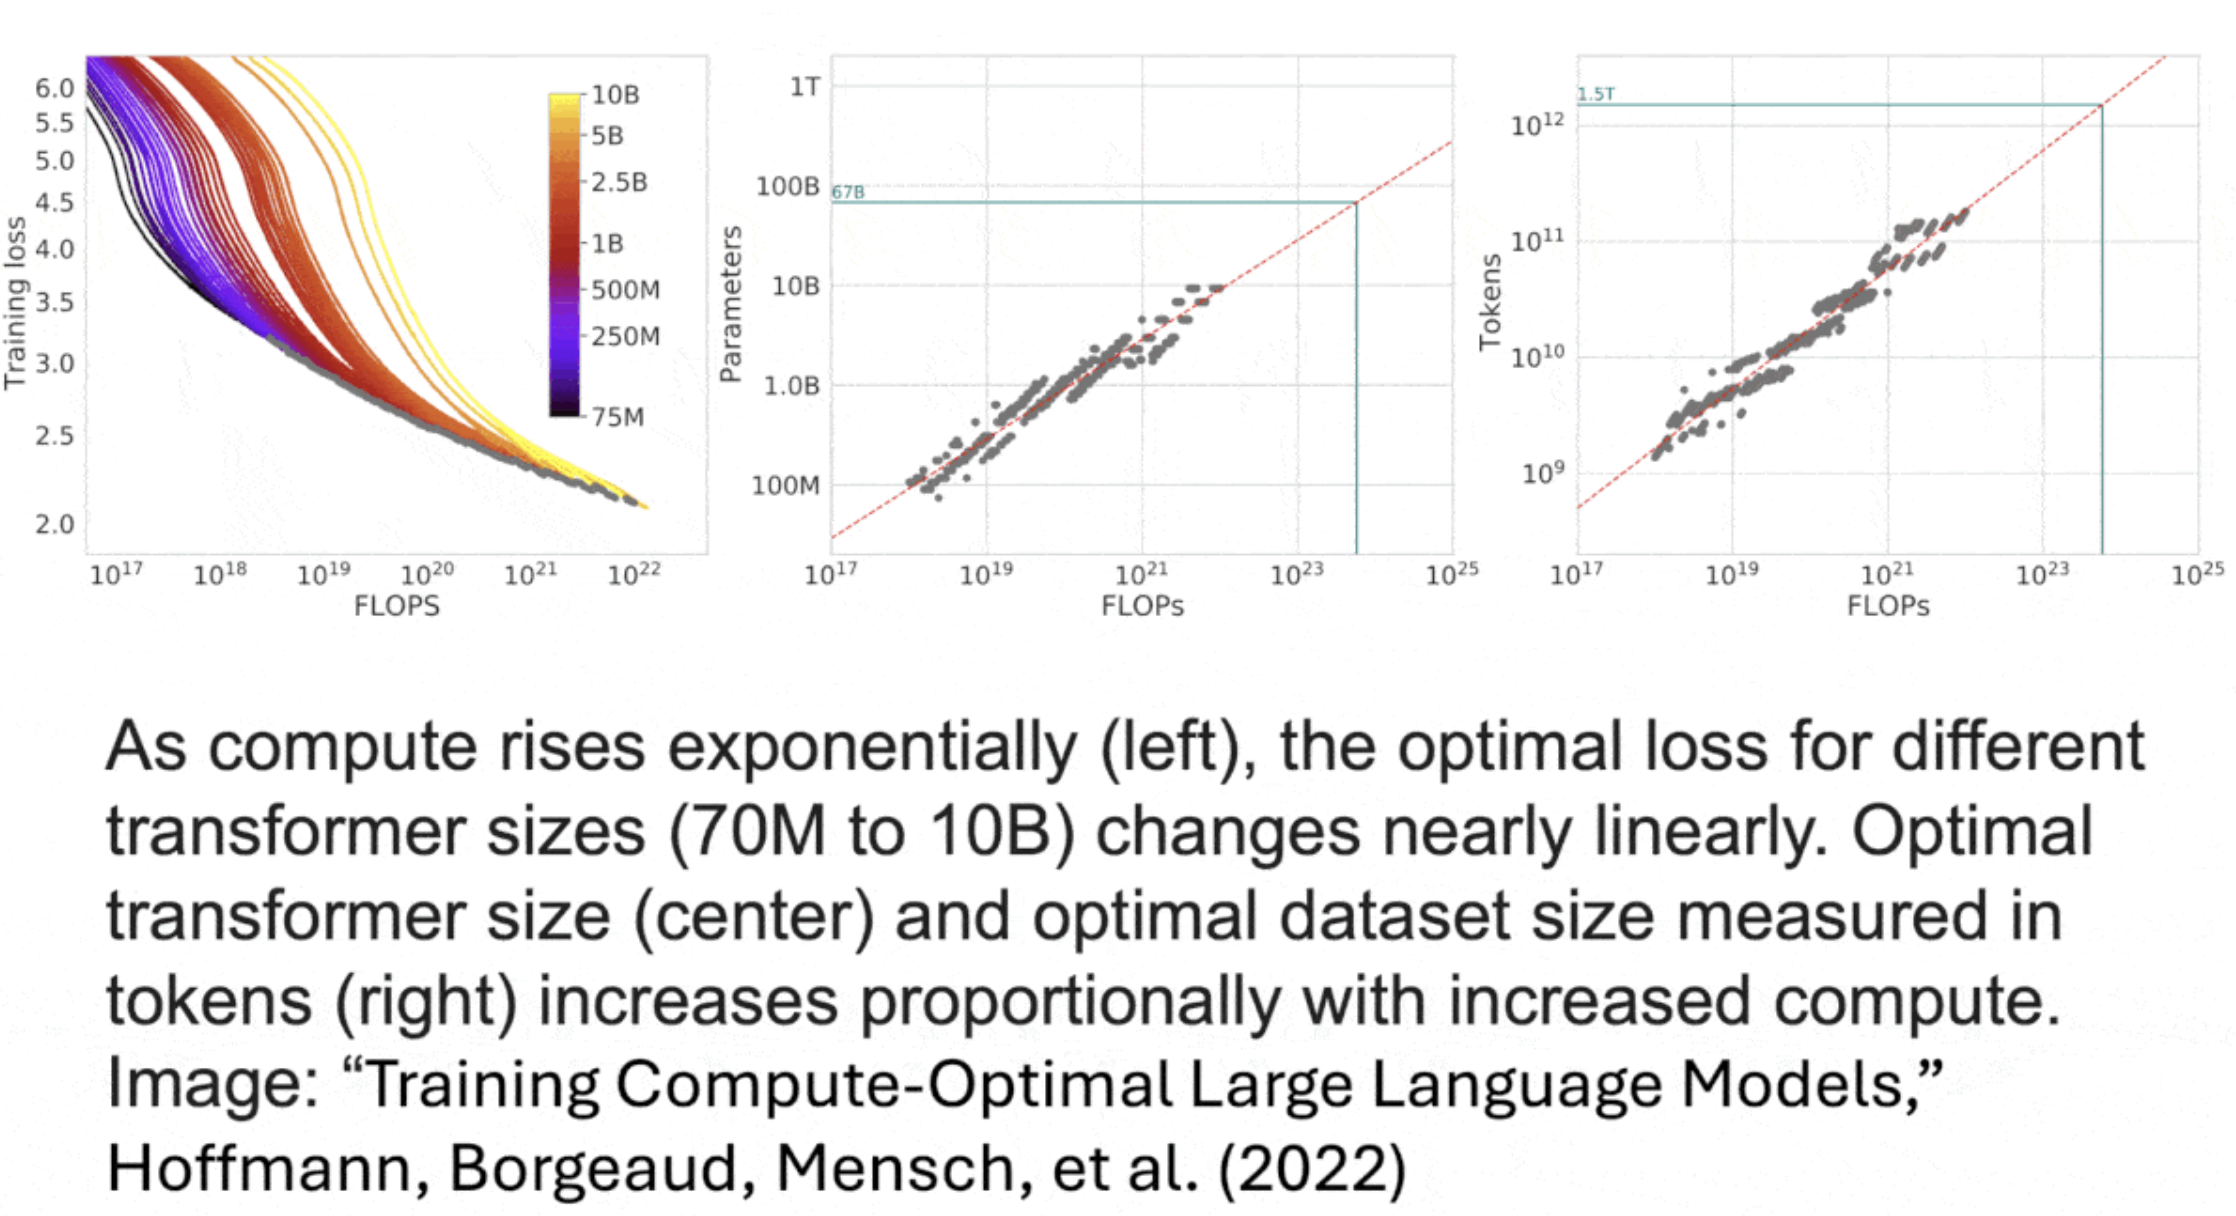
\includegraphics[width = 12cm]{./figure/linear,tokens,pars.png} 
\end{figure}

\vfill

\end{vbframe}

\begin{vbframe}{If there's one thing you should take away (2)}


\vfill

\begin{itemize}
	\item The original scaling laws were exclusively
        about \myblue{(pre)training}: What is the best model
        I can train given
        constraints such as compute budget.

\item This has shifted to \myblue{``joint optimization''} of training
        and testing: even if a trillion parameter model is the optimal
        model given training constraints, a much smaller
        model may be preferable since its so much cheaper at
        inference time.

\item Trend towards \myblue{systems of smaller models}, trend away
        from a single huge monolithic model.

\end{itemize}

\vfill

\end{vbframe}



\endlecture
\end{document}
